\documentclass{article}

% For COMP-579 final report (NeurIPS format, 4 pages max excluding references).
\usepackage[preprint]{neurips_2026}
\usepackage[utf8]{inputenc}
\usepackage[T1]{fontenc}
\usepackage{hyperref}
\usepackage{url}
\usepackage{booktabs}
\usepackage{amsfonts}
\usepackage{amsmath}
\usepackage{nicefrac}
\usepackage{microtype}
\usepackage{xcolor}
\usepackage{graphicx}
\usepackage{natbib} 

\title{Final Project Report: Self-Adaptive Success-Rate Reward Shaping (SASR)}

\author{
Yuchen Zhou \\
Group 115 \\
\texttt{yuchen.zhou2@mail.mcgill.ca}
\And
Junpeng Wen \\
Group 115 \\
\texttt{junpeng.wen@mail.mcgill.ca}
}

\begin{document}
\maketitle

\begin{abstract}
Sparse and delayed rewards remain a core obstacle in deep reinforcement learning. In this project we study Self-Adaptive Success Rate (SASR) reward shaping~\citep{ma2025sasr}, a method that augments environment rewards with a learned, state-dependent shaping signal derived from an evolving estimate of success probability. We use the reference implementation to reproduce behaviors on sparse-reward continuous-control benchmarks and extend the pipeline to discrete, image-based control in Super Mario Bros. This report summarizes the problem setting, the SASR mechanism, and our empirical findings.
\end{abstract}

\section{Introduction}
\label{sec:introduction}

Deep reinforcement learning excels in dense-reward settings but struggles with sparse rewards, where informative feedback is rare. This leads to sample-inefficient learning and exploration challenges. Common solutions include intrinsic exploration bonuses and reward shaping, which augments the environment reward with a policy-invariant bonus to accelerate learning.

This project focuses on Self-Adaptive Success Rate (SASR) reward shaping. SASR estimates a state-dependent success probability from past experience and uses a Thompson-sampling-inspired mechanism to provide an adaptive exploration bonus. We re-implemented SASR with a Soft Actor-Critic (SAC) backbone for continuous control and extended it to discrete, image-based control by performing density estimation in a learned CNN feature space.

Our goals are threefold: (1) reproduce SASR's key behaviors on sparse-reward continuous-control benchmarks; (2) understand the algorithmic choices behind its stability; and (3) evaluate its extension to pixel-based tasks alongside DQN and PPO baselines.

\section{Background}
\label{sec:background}

\paragraph{Sparse rewards and reward shaping.}
In sparse-reward tasks, the environment reward \(R^E\) is zero almost everywhere, making learning difficult. Reward shaping adds a shaping function \(F(s_t,a_t,s_{t+1})\) to \(R^E\) to provide denser feedback. Potential-based shaping \(F = \gamma\Phi(s_{t+1}) - \Phi(s_t)\) preserves optimal policies, but designing a good potential \(\Phi\) manually is challenging.

\paragraph{Beta-distributed success-rate shaping.}
SASR estimates the empirical success rate \(\hat p(s) = N_S(s)/(N_S(s)+N_F(s))\) using pseudo-counts \(N_S(s)\) and \(N_F(s)\) from successful and failed trajectories. To mitigate overconfidence, it samples a shaping reward from a Beta posterior:
\begin{equation}
r^S(s) \sim \mathrm{Beta}\!\big(N_S(s)+1,\; N_F(s)+1\big), \qquad
R^{\mathrm{SASR}}(s) = R^E(s) + \lambda\, f_{\mathrm{scale}}\!\big(r^S(s)\big),
\label{eq:sasr-core}
\end{equation}
where \(\lambda>0\) is a mixing weight and \(f_{\mathrm{scale}}\) maps \([0,1]\) to a practical reward range. This provides high-variance bonuses in underexplored regions and converges to a deterministic signal as data accumulates.

\paragraph{KDE with random Fourier features.}
Pseudo-counts are obtained via Kernel Density Estimation (KDE) on buffers \(\mathcal{D}_S, \mathcal{D}_F\):
\begin{equation}
N_X(s) \;=\; \frac{N}{|\mathcal{D}_X|}\sum_{s_j\in\mathcal{D}_X} \exp\!\Big(-\tfrac{\|s-s_j\|^2}{2h^2}\Big),\qquad X\in\{S,F\}.
\label{eq:kde}
\end{equation}
To avoid \(O(|\mathcal{D}_X|)\) cost, the Gaussian kernel is approximated with random Fourier features: \(K(s_i,s_j)\approx z(s_i)^\top z(s_j)\) with \(z(s) = \sqrt{2/M}\,\cos(\boldsymbol{W}^\top s + \boldsymbol{b})\). This reduces the count query to a single inner product.

\paragraph{Integration with RL.}
A trajectory is labeled a success if it contains any positive reward. The shaped reward from~\eqref{eq:sasr-core} is added to the TD target. For image-based inputs, KDE is performed in a learned CNN feature space to avoid the curse of dimensionality, and stored features are periodically refreshed to account for encoder drift during training.

\section{Methodology}
\label{sec:methodology}

Our methodology has three components: (i) reproducing the reference SASR implementation on a continuous-control benchmark, (ii) extending SASR to discrete, image-based control in Super Mario Bros, and (iii) comparing against PPO and DQN baselines on the same environment.

\subsection{SASR on Continuous Control (Reproduction)}

We use the authors' reference implementation of SASR with a SAC backbone~\citep{haarnoja2018sac} on \texttt{MountainCarContinuous-v0}, with all hyperparameters matching the original code. The SASR mechanism operates as described in Section~\ref{sec:background}: completed episodes are classified as success or failure based on whether any positive reward was observed, trajectory states are sub-sampled into $\mathcal{S}$ and $\mathcal{F}$ buffers, and RFF-accelerated KDE provides pseudo-counts that parameterise the Beta-distributed shaped reward added to the SAC TD target.

\subsection{Extension to Discrete Image-Based Control}

\paragraph{Environment and preprocessing.}
We use \texttt{gym-super-mario-bros}~\citep{gym-super-mario-bros} with the \texttt{SIMPLE\_MOVEMENT} action set (7 discrete actions). Observations pass through standard Atari-style preprocessing: 4-frame skip with max-pooling, grayscale resizing to $84 \times 84$, 4-frame stacking (final shape $4 \times 84 \times 84$), and $[0, 1]$ normalisation. We experiment with a \emph{sparse} variant where the agent receives only a terminal reward equal to its normalised forward distance.

\paragraph{From SAC to PPO backbone.}
Our initial implementation paired SASR with SAC-Discrete, mirroring the continuous-control pipeline. However, we observed consistent \emph{policy collapse}: the policy network would suddenly degenerate to outputting a single fixed action, ceasing all meaningful exploration. We attribute this to the off-policy replay buffer retaining stale shaped rewards computed under earlier density models, whose interaction with entropy-regularised SAC updates drives the policy toward a degenerate mode. We therefore adopt \textbf{PPO}~\citep{schulman2017proximal} as the backbone. PPO's clipped surrogate objective and on-policy updates proved substantially more stable.

\paragraph{SASR with PPO backbone.}
The architecture uses a shared CNN actor--critic: an Atari-style convolutional encoder mapping frames to a 512-dim feature vector, with separate linear heads for the categorical policy and scalar value. Because KDE in pixel space is infeasible, density estimation operates in this CNN feature space: at episode end, observations are encoded (under \texttt{no\_grad}) and sub-sampled into $\mathcal{S}$ or $\mathcal{F}$. After each PPO rollout, all observations are similarly embedded, KDE pseudo-counts are computed via RFF, and the Beta-sampled shaped reward is added to each step's reward \emph{before} GAE, propagating into both advantages and value targets.

Several modifications address challenges specific to this setting:
\begin{itemize}
    \item \textbf{Feature normalisation}: CNN features are $L^2$-normalised before KDE so that the bandwidth carries a stable cosine-distance interpretation as the encoder evolves.
    \item \textbf{FIFO buffer caps}: $\mathcal{S}$ and $\mathcal{F}$ are size-capped to bound memory and evict stale features. The pseudo-count multiplier uses actual buffer sizes instead of $t \cdot \phi$ to keep the Beta concentration well-calibrated under capping.
    \item \textbf{Adaptive success classification}: we augment the binary flag-based criterion with a quantile rule---a trajectory is labelled success if its terminal reward exceeds the top quartile of a rolling window---preventing the success buffer from remaining empty on hard levels.
    \item \textbf{Warm-up gating}: shaping is suppressed until $\mathcal{S}$ has accumulated enough entries, avoiding destabilisation from the uninformed $\mathrm{Beta}(1,1)$ prior.
\end{itemize}

\paragraph{Distributional lag.}
A key consideration is that the CNN representation drifts during training, but features stored in $\mathcal{S}$ and $\mathcal{F}$ reflect the encoder state at insertion time. This \emph{distributional lag} means stale stored features and freshly extracted query features inhabit different manifolds, degrading the discriminative power of the success-rate signal. The FIFO cap and $L^2$-normalisation partially mitigate this by bounding feature age and stabilising scale, but do not eliminate the geometric mismatch.

\paragraph{Baselines.}
We compare against two baselines using the same preprocessing pipeline. \textbf{Dueling Double DQN}~\citep{mnih2015dqn} uses a similar CNN backbone split into value and advantage streams, trained with $\epsilon$-greedy exploration and experience replay. \textbf{PPO}~\citep{schulman2017proximal} uses the identical shared CNN actor--critic as the SASR method (without shaping), trained with GAE-$\lambda$, clipped surrogate objective, entropy bonus, and learning-rate annealing.


\section{Experimental Results}
\label{sec:results}

We evaluate all three agents on \texttt{SuperMarioBros-1-1-v1} with sparse rewards. Each agent is trained for approximately $1\text{M}$ environment steps. Figure~\ref{fig:training-curves} shows the episodic return during training; Table~\ref{tab:eval} summarises deterministic-policy evaluation after training.

\begin{figure}[h]
  \centering
  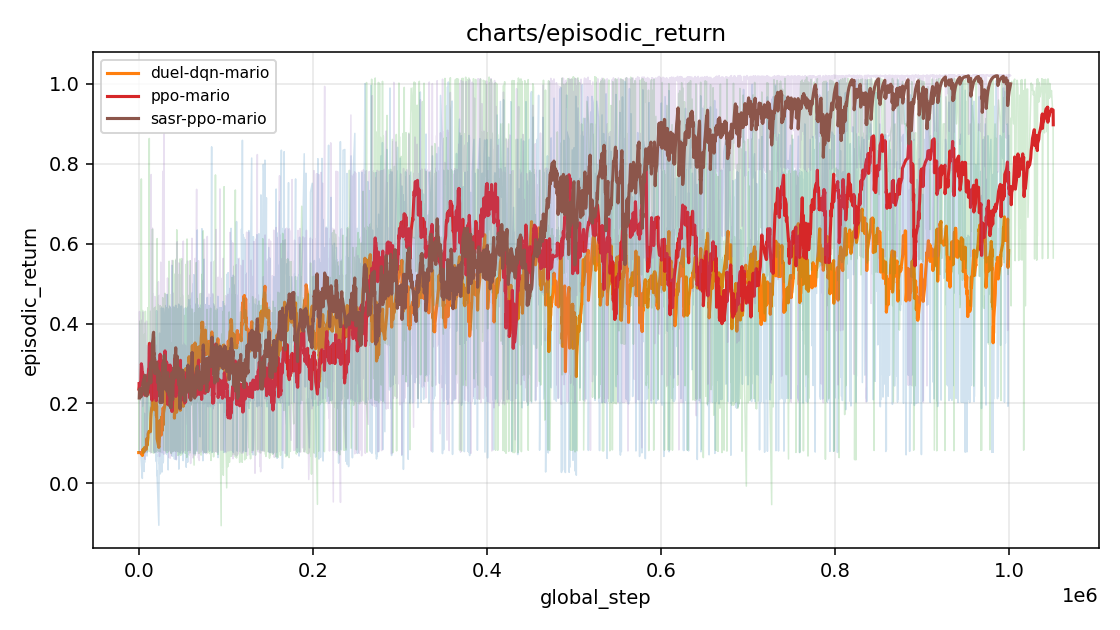
\includegraphics[width=0.8\linewidth]{charts__episodic_return.png}
  \caption{Episodic return vs.\ global step for Dueling DQN, PPO, and SASR+PPO on Super Mario Bros 1-1 (smoothed with EMA $\alpha=0.9$; raw values shown in background). SASR+PPO reaches the maximum return ($\approx1.0$) around 800k steps, while PPO plateaus near $\approx0.8$ and DQN near $\approx0.6$.}
  \label{fig:training-curves}
\end{figure}

\begin{table}[h]
  \centering
  \caption{Deterministic evaluation on Super Mario Bros 1-1 after training. Position denotes normalised forward distance ($0$--$1$); $1.0$ means completing the level.}
  \label{tab:eval}
  \begin{tabular}{lccc}
    \toprule
    Agent & Position & Level Complete & Mean Return \\
    \midrule
    Dueling DQN & $0.22$ & No & $\sim\!0.6$ \\
    PPO & $0.76$ & No & $\sim\!0.8$ \\
    SASR + PPO & $\mathbf{1.00}$ & \textbf{Yes} & $\sim\!\mathbf{1.0}$ \\
    \bottomrule
  \end{tabular}
\end{table}

\paragraph{DQN.} The Dueling Double DQN agent learns slowly and plateaus at an episodic return of $\approx0.6$, reaching only about 22\% of the level. Its $\epsilon$-greedy exploration is insufficient to discover the extended action sequences needed to advance through later sections of the level.

\paragraph{PPO.} PPO shows substantially stronger learning, with episodic return climbing steadily and reaching $\approx0.8$ by 1M steps. The agent navigates to approximately 76\% of the level but does not complete it within the training budget. PPO's on-policy learning and entropy bonus provide better exploration than DQN, yet the sparse reward signal still limits the agent's ability to discover successful trajectories through the final portion of the level.

\paragraph{SASR + PPO.} The SASR-PPO agent is the only method that successfully completes the sparse-reward task. By constructing a density model in the CNN feature space, the agent is continuously drawn toward novel states that share characteristics with previously successful trajectories. This intrinsic motivation provides a dense learning signal that allows the agent to cross the bottleneck where standard PPO stalls, ultimately reaching a level progression of $1.0$ and successfully completing the entire journey to the flag.

\paragraph{Effect of distributional lag.} Applying KDE in a dynamically updating feature space risks distributional lag: stored features from early successes can drift out of alignment with the current encoder. In practice this mismatch only induces transient variance in the episodic returns, and the agent still converges reliably. We attribute this robustness to $L^2$-normalisation and strict FIFO buffer caps, which bound feature age and stabilise scale, together with adaptive success classification, which keeps a steady influx of fresh success features and prevents the density model from locking into stale representations.

\section{Conclusion and Future Work}
In this project, we successfully extended the SASR reward shaping method to discrete, image-based environments by integrating it with a PPO backbone and performing density estimation in a learned CNN feature space. Our SASR-PPO agent overcame the sparse reward challenges in Super Mario Bros, completing the level where standard PPO and DQN baselines stalled. We mitigated the inherent distributional lag using $L^2$-normalisation and adaptive buffer management. 

For future work, it would be interesting to explore mechanisms that explicitly align historical features with the current encoder (e.g., representation momentum or distillation) and to evaluate the method's generalisation across a wider suite of procedurally generated levels.

\section*{Contributions and Acknowledgements}

\paragraph*{Contributions.} The work was equally shared. Junpeng Wen led the integration of SASR with the PPO backbone, including architecture design and experimentation. Yuchen Zhou implemented the DQN baseline and the sparse reward environment. Both authors contributed to reproducing the original SASR algorithm, writing the report, and project management.

\paragraph*{Acknowledgements.} We thank the authors of \citet{ma2025sasr} for their open-source code. We also acknowledge the maintainers of \texttt{gym-super-mario-bros}, \texttt{Stable-Baselines3}, and \texttt{PyTorch}.

{
\small
\bibliographystyle{plainnat}
\bibliography{references} 
}

\end{document}